\section{Die Ableitung 1. Grades}
Die Ableitung 1. Grades beschreibt die Steigung an einem bestimmten Punkt der Funktion. In der Abbildung \ref{fig:00_steigung_an_punkt}
wird eine Funktion $f(x)$ (in grün) gegeben. Die Steigung $f'(x)$ an einem bestimmten Punkt $x$ ist rot markiert.
Die Ableitung selbst ist wiederum eine Funktion und kann über diverse Ableitungsregeln aufgrund der gegebenen Funktion
selbst gebildet werden.
\begin{figure}[h!]
    \begin{center}
        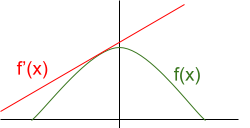
\includegraphics[width=0.4\linewidth]{../common/02_appendix/00_resources/00_derivation.png}
    \end{center}
    \caption{Steigung an einem bestimmten Punkt der Funktion $f(x)$}
    \label{fig:00_steigung_an_punkt}
\end{figure}

\section{Die partielle Ableitung}
Ist der Input einer Funktion mehrdimensional, das heisst, die Funktion $f$ ist abhängig von mehreren Variablen, dann
kann die Ableitung jeweils lediglich nach einer Variablen gebildet werden. Die übrigen Variablen werden als konstant
angesehen. In dem Fall beschreibt die partielle Ableitung die Steigung an einem bestimmten Punkt der abgeleiteten
Dimension. Es sei die Funktion $f(x, z) = x^2 + z^2 + 10$ gegeben. Diese wird nun partiell nach $x$ sowie
nach $z$ abgeleitet.
\begin{align}
    f^x(x, z) = 2x\\
    f^z(x, z) = 2z
\end{align}
Die hierbei angewendete Ableitungsregel heisst Potenzregel und lautet\\$f(x) = x^n \longrightarrow f'(x) = n \cdot x^{n-1}$.

\section{Die Kettenregel}
Schaut man sich
